\documentclass[withoutpreface,bwprint]{cumcmthesis} 
\usepackage{subcaption} % 子标题
\usepackage[linesnumbered, ruled, lined,boxed,commentsnumbered]{algorithm2e}[1]
\renewcommand{\algorithmcfname}{算法5 -}  %<---细节与重点
\SetKwInput{KwIn}{输入}  %<---细节与重点
\SetKwInput{KwOut}{输出}  %<---细节与重点
\title{\LaTeX 数学建模论文模板2.0}

\begin{document}
\maketitle
 \begin{abstract}

    这里是摘要。

\keywords{关键词1\quad  关键词2\quad   关键词3\quad  关键词4}
\end{abstract}

\section{问题背景与重述}
	
\subsection{问题背景}

\subsection{问题重述}

我们所需要解决的问题如下。

\textbf{问题一:}

\textbf{问题二:}

\textbf{问题三:}

\textbf{问题四:}

\section{问题分析}

\subsection{问题一分析}

在这里写问题一的分析。

\subsection{问题二分析}

在这里写问题二的分析。

\subsection{问题三分析}

在这里写问题三的分析。

\subsection{问题四分析}

在这里写问题四的分析。

\section{模型假设}

\begin{enumerate}
    \item 这里是第一条假设。
    \item 这里是第二条假设。
    \item 这里是第三条假设。
    \item 这里是第四条假设。
\end{enumerate}

\section{符号说明}

\begin{table} [ht]
    \centering 
    \begin{tabular} {  p{0.15\textwidth}<{\centering}p{0.6 \textwidth}<{\centering}p{0.15\textwidth}<{\centering}  }
        \toprule
        \textbf{符号}&\textbf{说明}&\textbf{单位}\\
        \midrule
        $S$&市区到机场的距离&m\\
        \bottomrule
    \end{tabular}
\end{table}


\section{模型的建立与求解}

\subsection{问题一模型建立与求解}

针对问题1,建立了模型1。

其中,公式的书写方式如下。
\begin{equation}
    \label{eq1}
    {\rm{e}}^{i\theta}=\cos\theta+i\sin\theta.
\end{equation}
公式\ref{eq1}就是大名鼎鼎的Euler公式。

\subsection{问题二模型建立与求解}

针对问题2,建立了模型2。

在论文中可能需要插入图片,在这里插入图片的方式如下。
\begin{figure}[htbp] 
    \centering 
    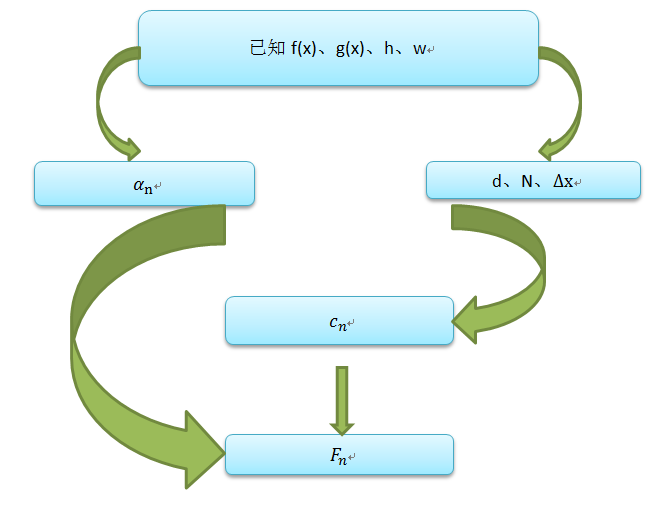
\includegraphics[width=0.4\textwidth]{f1}
    \caption{插入一张图}
    \label{fig.1}
  \end{figure}
\begin{figure}[htbp]
    \centering
    \begin{minipage}[c]{0.3\textwidth}
        \centering
        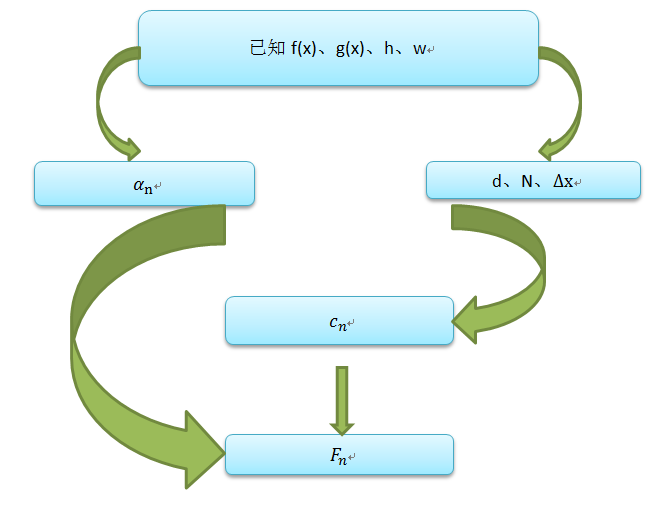
\includegraphics[width=0.95\textwidth]{f1}
        \subcaption{流程图}
        \label{fig:sample-figure-a}
    \end{minipage}
    \begin{minipage}[c]{0.3\textwidth}
        \centering
        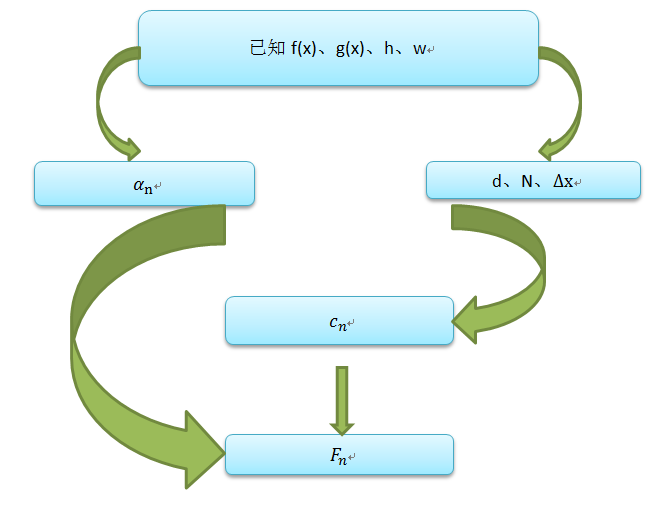
\includegraphics[width=0.95\textwidth]{f1}
        \subcaption{流程图}
        \label{fig:sample-figure-b}
    \end{minipage}
    \begin{minipage}[c]{0.3\textwidth}
        \centering
        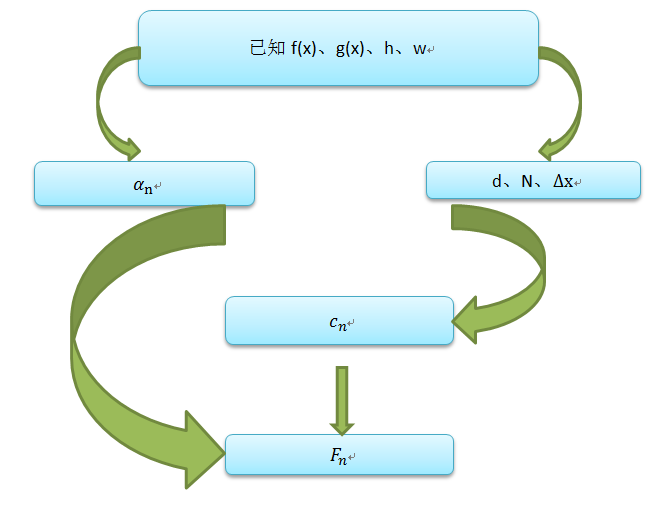
\includegraphics[width=0.95\textwidth]{f1}
        \subcaption{流程图}
        \label{fig:sample-figure-c}
    \end{minipage}
    \caption{多图并排示例}
    \label{fig:sample-figure}
\end{figure}

\subsection{问题三模型建立与求解}

模型求解算法:

\begin{algorithm}[H]
    \renewcommand{\thealgocf}{3}     %<---细节与重点
    \SetAlgoLined
    \KwIn{路径集合 $\mathcal{W} $ }
   
    \KwOut{ 节点的嵌入式表示 $\mathbb{R}$ }
    
    \ForEach{$v_j$ in $\mathcal{W}_{v_i}$}
    {
     \ForEach{$u_k \in \mathcal{W}_{v_i}  \left[ j-w : j +w  \right] $}
     {
      $J(\Phi) = - log P\left( u_k | \Phi  ( v_j) \right)$ \;
      $\Phi = \Phi - \alpha * \frac{\partial J}{\partial \Phi }$ \;
  
     }
    }  
    \caption{利用跳元(Skip-Gram)模型更新节点嵌入参数}
   \end{algorithm}
\subsection{问题四模型建立与求解}

最优化模型:

\textbf{目标函数:}
\begin{equation}
    \theta^{\ast}=\mathop{\arg\max}\limits_{\theta} \sum _{i=1}^{n} L\left(y_i,f(x_i)\right)+\lambda \Omega (\omega)
\end{equation}

\textbf{约束条件:}

\begin{equation}
    \text{s.t.}\begin{cases}
        1111\\
        2222\\
        3333
    \end{cases}
\end{equation}

模型求解过程:

\textbf{Step1:初始化:}

\textbf{Step2:计算基尼系数:}



\section{结果的分析与检验}

\subsection{问题的结果}

在这里写问题的结果。

\subsection{模型的检验}

在这里写对模型的检验。

\section{模型的优缺点分析}

\subsection{模型的优点}

该模型具有如下的优点。
\begin{itemize}
    \item 优点1;
    \item 优点2;
    \item 优点3。
\end{itemize}

\subsection{模型的缺点}

与此同时,该模型也具有如下的缺点。
\begin{itemize}
    \item 缺点1;
    \item 缺点2。
\end{itemize}

\subsection{模型的改进}

同时,在这里给出进一步优化模型的思路。


\begin{thebibliography}{9}%宽度9
    \bibitem[1]{liuhaiyang2013latex}
    刘海洋.
    \newblock \emph{\LaTeX {}入门}\allowbreak[J].
    \newblock 电子工业出版社, 北京, 2013.
    \bibitem[2]{mathematical-modeling}
    全国大学生数学建模竞赛论文格式规范 (2020 年 8 月 25 日修改).
\end{thebibliography}

\newpage
%附录
\begin{appendices}

    \section{所用软件}
    
    
    \section{问题一}
    
    \begin{lstlisting}[style=matlab,title={MATLAB code}]
% Euler method for the ODE model
% u'(x)=x^2+x-u, x in [0,1]
% Initial condition: u(0)=0 ;
% Exact solution: u(x)=-exp(-x)+x^2-x+1.
clear all;  clf
h=0.1;
x=0:h:1;
N=length(x)-1;
u(1)=0;                        % initial value
fun=@(t,u) t.^2+t-u;           % RHS

for n=1:N
    u(n+1)=u(n)+h.*fun(x(n),u(n));
end

ue=-exp(-x)+x.^2-x+1;          % exact solution
plot(x,ue,'b-',x,u,'r+','LineWidth',1)
legend('Exact','Numerical','location','North')
%title('Euler method','fontsize',12)
set(gca,'fontsize',12)
xlabel('x','fontsize',16), ylabel('u','fontsize',16,'Rotation',0)
\end{lstlisting}


\begin{lstlisting}[style=python,title={Python code}]
#PythonDraw.py
import turtle as t
t.setup(650, 350, 200, 200)
t.penup()
t.fd(-250)
t.pendown()
t.pensize(25)
t.pencolor("purple color")
t.seth(-40)
for i in range(4):
    t.circle(40, 80)
    t.circle(-40, 80)
t.circle(40, 80/2)
t.fd(40)
t.circle(16, 180)
t.fd(40 * 2/3)
t.done()
    \end{lstlisting}
    \end{appendices}

\end{document} 